% ****** Start of file apssamp.tex ******
%
%   This file is part of the APS files in the REVTeX 4.1 distribution.
%   Version 4.1r of REVTeX, August 2010
%
%   Copyright (c) 2009, 2010 The American Physical Society.
%
%   See the REVTeX 4 README file for restrictions and more information.
%
% TeX'ing this file requires that you have AMS-LaTeX 2.0 installed
% as well as the rest of the prerequisites for REVTeX 4.1
%
% See the REVTeX 4 README file
% It also requires running BibTeX. The commands are as follows:
%
%  1)  latex apssamp.tex
%  2)  bibtex apssamp
%  3)  latex apssamp.tex
%  4)  latex apssamp.tex
%
\documentclass[%
 reprint,
%superscriptaddress,
%groupedaddress,
%unsortedaddress,
%runinaddress,
%frontmatterverbose, 
%preprint,
%showpacs,preprintnumbers,
%nofootinbib,
%nobibnotes,
%bibnotes,
 amsmath,amssymb,
 aps,
%pra,
%prb,
%rmp,
prstab,
%prstper,
%floatfix,
]{revtex4-1}

\usepackage{graphicx}% Include figure files
\usepackage{dcolumn}% Align table columns on decimal point
\usepackage{bm}% bold math
%\usepackage{hyperref}% add hypertext capabilities
%\usepackage[mathlines]{lineno}% Enable numbering of text and display math
%\linenumbers\relax % Commence numbering lines
\usepackage{color}
\usepackage{siunitx}
\usepackage{url}

%\usepackage[showframe,%Uncomment any one of the following lines to test 
%%scale=0.7, marginratio={1:1, 2:3}, ignoreall,% default settings
%%text={7in,10in},centering,
%%margin=1.5in,
%%total={6.5in,8.75in}, top=1.2in, left=0.9in, includefoot,
%%height=10in,a5paper,hmargin={3cm,0.8in},
%]{geometry}

\DeclareFontFamily{U}{wncy}{}
\DeclareFontShape{U}{wncy}{m}{n}{<->wncyr10}{}
\DeclareSymbolFont{mcy}{U}{wncy}{m}{n}
\DeclareMathSymbol{\Sh}{\mathord}{mcy}{"58} 

\newcommand{\q}[2]{\ensuremath{#1\ \mathrm{#2}}} % quantity with units

\begin{document}

\title{Effects of pulsed hollow electron lens operation on the beam core in HL-LHC: \\First experimental studies and simulations.}% Force line breaks with \\
\thanks{Fermilab is operated by Fermi Research Alliance, LLC under
	Contract No.~DE-AC02-07CH11359 with the United States Department of
	Energy. This work was partially supported by the US DOE LHC
	Accelerator Research Program (LARP) and by the European FP7 HiLumi
	LHC Design Study, Grant Agreement 284404.}

\author{Miriam Fitterer}
 \email{mfittere@fnal.gov}
\author{Giulio Stancari}%
\author{Alexander Valishev}%
\affiliation{Fermi National Accelerator Laboratory, Batavia, Illinois, USA
% This line break forced with \textbackslash\textbackslash
}%

\author{Giulia Papotti}
\author{Stefano Redaelli}
\author{Daniel Valuch}
\affiliation{CERN, Geneva, Switzerland}%

\date{\today}% It is always \today, today,
             %  but any date may be explicitly specified

\begin{abstract}
In the HL-LHC a considerable amount of energy is stored in the beam tails due to the high beam intensity and an overpopulation of the tails compared to a Gaussian distribution. To control and clean the tail population, the installation of two hollow electron lenses, one per beam, is considered. Beside the DC operation, also a pulsed operation of the hollow electron lens is considered, which would considerably increase the diffusion speed by putting noise on the halo particles. In the ideal case, that is in case of no field at the beam core, only the halo particles are excited while leaving the core unperturbed. The picture though changes, if a residual field is present also at the location of the beam core putting noise also on the beam core. In this paper we present for estimates of the residual field at the beam core expected from the HL-LHC hollow electron lens and first experimental results of the effect of this excitation on the beam core together with the supporting simulations.
\end{abstract}

% PACS 2008:
% 29.20.db Storage rings and colliders

\pacs{29.20.D-}% PACS, the Physics and Astrtheonomy
                             % Classification Scheme.
%\keywords{Suggested keywords}%Use showkeys class option if keyword
                              %display desired
\maketitle

%\tableofcontents

\section{Introduction\label{sec:intro}}%force line break with \protect\\
Considering past, current and future high energy and intensity colliders, each new machine has represented a considerable leap in stored beam energy with rising values for future accelerators and colliders (see Table~\ref{tab:stored_energy}). 
\begin{table*}
	\caption{\label{tab:stored_energy}%
		Stored beam energy for different past, present and future colliders. Each new machine represents a leap in stored beam energy.
	}
	\begin{ruledtabular}
		\begin{tabular}{lccccc}
			Collider& Tevatron (protons) \cite{tevatron} & LHC 2016 \cite{chamonix2017param}
			& LHC nominal \cite{lhc_design} & HL-LHC \cite{hlcdr} & FCC \cite{fcc_param_2017} \\
			\colrule
			Beam energy [TeV] & 0.98 & 6.5 & 7.0 & 7.0 & 50.0\\
			Number of bunches & 36 & 2220 & 2808 & 2748 & ? \\
			Number of particles per bunch & $2.90\times 10^{11}$ & $1.15\times 10^{11}$ & $1.15\times 10^{11}$ & $2.2\times 10^{11}$ & $1.0\times 10^{11}$\\
			Stored beam energy [MJ] & 1.6 & 265.9 & 362.2 & 678.0 & 8400 \\
		\end{tabular}
	\end{ruledtabular}
\end{table*}
Recent measurements at the LHC furthermore show that the tails of the transverse beam distribution are overpopulated compared to a Gaussian distribution resulting in a considerable amount of energy being stored in the beam tails alone. In case of the LHC explicitly around 5\% of the beam population is stored in the tails above 3.5~$\sigma$ compared to 0.22\% in case of a Gaussian distribution leading to 19~MJ of stored energy in the tails in case of nominal LHC parameters and 34~MJ in case of HL-LHC~\cite{helreview_valentino}.

All of the above reasons lead to the conclusion that a mechanism is needed to deplete the beam tails in a controlled manner (see for example \cite{helreview} in case of HL-LHC). The most obvious idea is to decrease the collimator gaps or scrape the tails with a collimator type device. The minimum gap size of the collimators is however limited by the impedance of the machine and small enough gap sizes can therefore not be reached without risking an instability of the beam. Other mechanisms must therefore be found to actively deplete the tails.

Most promising are methods, which considerably increase the diffusion speed in the region of the halo particles while leaving the beam core unperturbed. The diffusing halo particles are then intercepted by the collimation system and removed (see Fig.~\ref{fig:active_halo_control} for illustration). This concept is also referred to as active halo control compared to a passive system, which only intercepts the halo particles without actively controlling the diffusion speed. Currently, the LHC collimation system is a passive halo control system. 
\begin{figure}[h]
	\begin{minipage}[t]{0.49\linewidth}
		\centering
		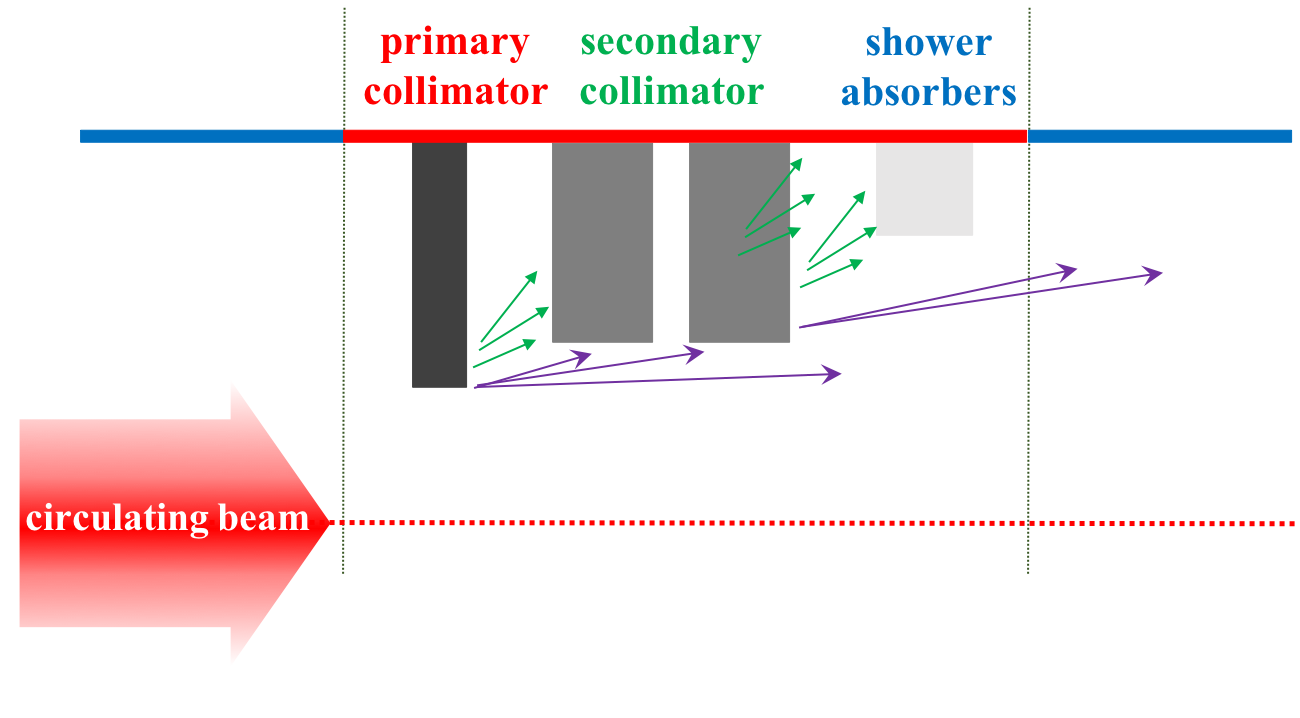
\includegraphics[width=1.0\linewidth]{passive_halo_control.png}
	\end{minipage}
	\begin{minipage}[t]{0.49\linewidth}
		\centering
		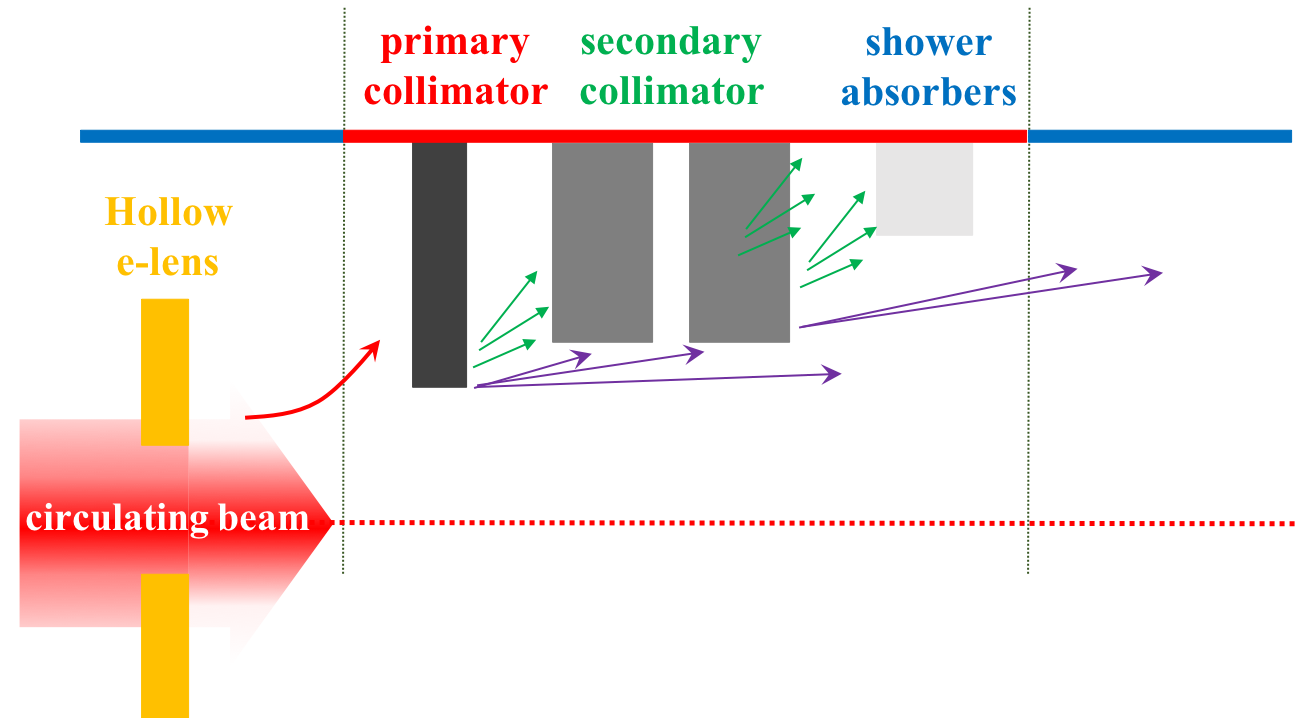
\includegraphics[width=1.0\linewidth]{active_halo_control.png}
	\end{minipage}	
	\caption{\label{fig:active_halo_control} Sketch of passive halo control as with the collimation system (top) and active halo control using in addition for example a hollow electron lens (HEL) to control the diffusion speed in the region tail region without affected the beam core (bottom). \textcolor{red}{Any acknowledgement needed for the plots?}.}
\end{figure}

In view of the need of an active halo control system for LHC and HL-LHC in particular and in general for future high power accelerators, different methods have been studied in the last recent years \cite{helreview_bruce}, of which the HEL is considered the superior device at least in case of the HL-LHC \cite{helreview} and is also considered for other future high energy colliders like HE-LHC and FCC-hh \cite{helhcparam2011,fccparam2016}.

The beneficial effect of an active halo control system is however abrogated if also the beam core is affected as this would ultimately lead to a degradation of the performance due to losses of particles in the core region and emittance growth. In this paper, we will concentrate on this aspect in view of future HEL to be installed in the HL-LHC. We will summarize possible sources of perturbations of the beam core concentrating in particular on the case of pulsed operation and with the focus on the beam experiments at the LHC performed in this context.

This paper is structured as follows: Section~\ref{sec:hel} gives an introduction to the concept of HELs and summarizes the design parameters of the HL-LHC HEL. Section~\ref{sec:core} is dedicated to describing the sources of a residual field from the HEL in the core region. Section~\ref{sec:exp_sum}--\ref{sec:exp_sim} describes then in detail the two beam experiments conducted at the LHC to study the effect on the beam core in case of a pulsed HEL operation. This includes the detailed analysis of the observed losses, emittance and transverse beam distribution changes. To the knowledge of the authors, the observed distribution changes presented in this paper have never been measured before in the context of a resonant excitation. A resonant excitation has been previously studied at the Tevatron in the context of the HEL experiments \cite{hel_tevatron_stancari} and the abort gap cleaning used in operation \cite{hel_tevatron_abortgap_zhang}. Both studies however only concentrated on the losses and emittance changes without measuring the detailed changes of the distribution itself. In addition, the presented experiments also provide scalings of the losses and emittance growth with the excitation amplitude. This allows to provide first tolerances for the residual field of the HL-LHC HEL at the beam core and also to compare the obtained results with simulations and thus benchmark the same.

\section{Hollow electron lens for HL-LHC\label{sec:hel}}
\subsection{General Overview\label{sec:hel:intro}}
In general, electron lenses are DC or pulsed low energy electron beams. The electron beam is generated in an electron gun, then guided and confined by strong solenoids and finally dumped onto a collector. Exemplary for the conceptual design of all electron lenses, the HL-LHC HEL is shown in Fig.~\ref{fig:hel_layout}.
\begin{figure}[h]
	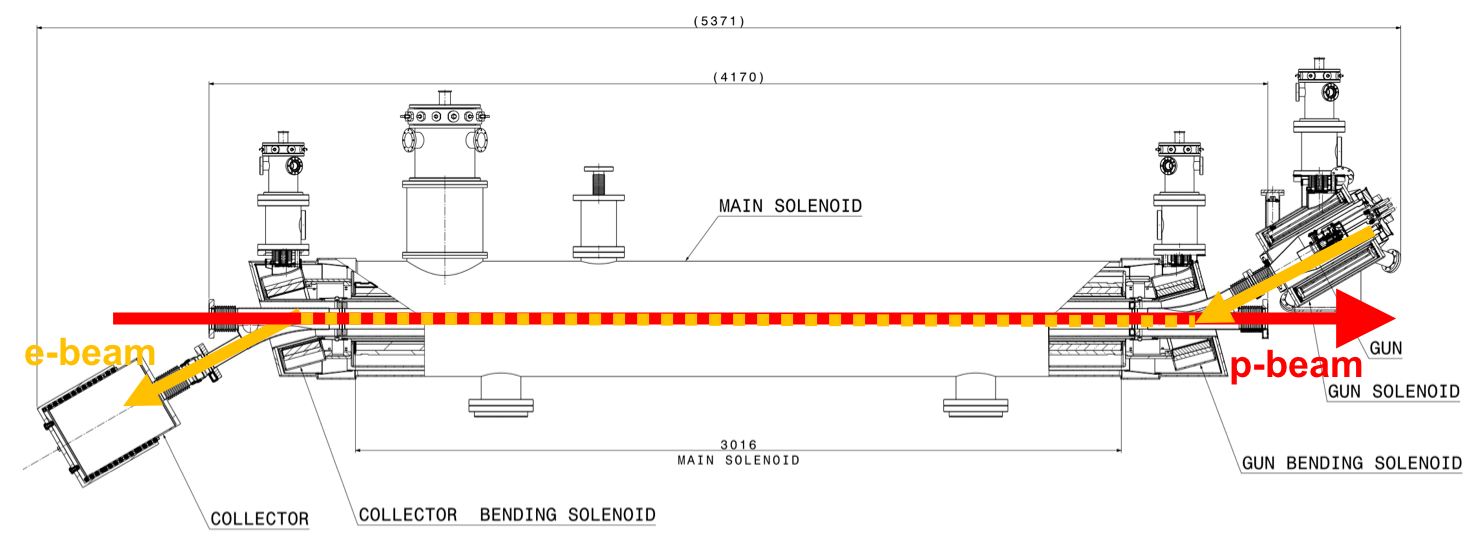
\includegraphics[width=1.0\linewidth]{hel_layout_epbeam}% Here is how to import EPS art
	\caption{\label{fig:hel_layout} Layout of HL-LHC HEL.}
\end{figure}
The circulating beam, in case of the LHC the proton beam, is then affected by the electromagnetic field of the electron beam. For the application of active halo control, the electron beam needs to generate an electromagnetic field at the location of the halo particles while leaving the core untouched. This can be achieved by using a uniform hollow distribution in radius $r=\sqrt{x^2+y^2}$ with inner radius $R_1$ and outer radius $R_2$. In this case, the circulating proton beam experiences a radial kick $\theta(r)$
\begin{equation}\label{eq:field_1}
\theta(r)=\frac{f(r)}{(r/R_2)}\cdot \theta_{\rm max},
\end{equation}
where $f(r)$ is a shape function with
\begin{equation}\label{eq:field_2}
f(r) =
\begin{cases} 0 &,\quad r< R_1,\\
\frac{r^2-R_1^2}{R_2^2-R_1^2} &,\quad R_1 \leq r < R_2,\\
1 &,\quad R_2 \leq r
\end{cases}
\end{equation}
and $\theta_{\rm max}=\theta(R_2)$ is the maximum kick angle given by
\begin{equation}
\theta_{\rm max} = \theta(R_2) = \frac{2LI_T(1\pm\beta_e\beta_p)}{4\pi\epsilon_0  \cdot \left(\frac{q}{p_0}\right)_p \cdot \beta_e\beta_p c^2}\cdot\frac{1}{R_2},
\end{equation}
where $L$ is the length of the e-lens, $I_T$ the total electron beam current, $\beta_{e}$ and $\beta_{p}$ the relativistic $\beta$ of electron and proton beam, $\frac{q}{p_0}=\left(B\rho\right)_p$ the magnetic rigidity for the reference particle, $c$ the speed of light and $\epsilon_0$ the vacuum permittivity.
\begin{figure}[b]
	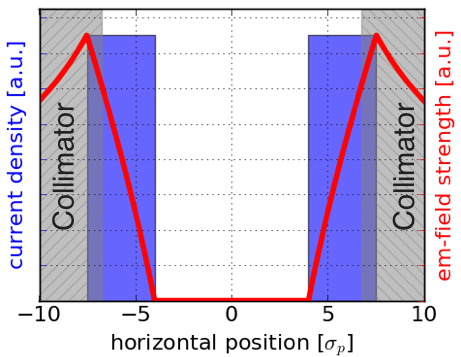
\includegraphics[width=0.8\linewidth]{hel_field}% Here is how to import EPS art
	\caption{\label{fig:hel_field} Illustration of the hollow electron beam distribution (blue), the kick experienced by the proton beam (red) and the collimators (gray).}
\end{figure}
\begin{table}[t]
	\caption{\label{tab:hel_param}%
		HL-LHC hollow electron lens parameters as in~\cite{hel_cdr}.
	}
	\begin{ruledtabular}
		\begin{tabular}{lcc}
			Geometry & Value& Unit\\
			\colrule
		Length $L$    &  3 & m\\
		Desired range of scraping positions\footnote{$\sigma$ denotes here the Beam sigma and not the collimation $\sigma$ which assumes a normalized emittance of 3.5~$\mu$m.} & 4-8 &$\sigma_p$\\
		\colrule
		Magnetic fields & & \\
		\colrule
		Gun solenoid, $B_g$ & 0.2-0.4 & T\\
		Main solenoid, $B_m$ & 2-6 & T\\
		Collector solenoid, $B_c$ & 0.2-0.4 & T\\
		Compression factor ($k=\sqrt{B_m/B_g}$) & 2.2-5.5 & -\\
		\colrule
		Electron gun & & \\
		\colrule
		Peak yield $I_e$ at 10~keV & 5.0 & A\\
		Gun perveance $P$ & 5 & $\mu$perv\\
		Inner/outer cathode radius, $R_1/R_2$ & 6.75/12.7 & mm\\
		\colrule
		High voltage modulator & & \\
		\colrule
		Cathode-anode voltage & 10.0 & kV\\
		Rise time (10\%-90\%) & 200 & ns \\
		Repetition rate & 35 & kHz
		\end{tabular}
	\end{ruledtabular}
\end{table}

The distribution together with the resulting kick are illustrated in Fig.~\ref{fig:hel_field}. The $\pm$-sign represents the two cases of the electron beam traveling in the direction of the proton beam ($v_e v_p>0$) leading to ``$-$" or in the opposite direction ($v_e v_p<0$) leading to ``$+$". For hollow electron beam collimation, electron and proton beam travel in opposite directions. Assuming HL-LHC and HEL design parameters (Table~\ref{tab:hel_param}--\ref{tab:hllhc_param}) the maximum kick of the HEL is:
\begin{equation}
\theta_{\rm max,B1} = 392~\rm{nrad}
\end{equation}
%\begin{eqnarray}
%\theta_{\rm max,B1} = 392~\rm{nrad},\\
%\theta_{\rm max,B2} = 341~\rm{nrad}.
%\end{eqnarray}
for an inner radius $R_1=4\sigma_p$, outer radius $R_2=7.5\sigma_p$ and a peak current of $I_e=$\SI{5.0}{A}. Similar values are obtained for Beam~2.

\subsection{Operation modes and effects on the beam core\label{sec:hel:core}}
As depicted in Fig.~\ref{fig:hel_field} and in evidence from Eq.~\ref{eq:field_1}--\ref{eq:field_2}, the field at the beam core vanishes in the ideal case. Effects on the beam core thus only arise in case of imperfections, where possible sources are the bends of the HEL, as the electron beam crosses directly the proton beam, and distortions in the electron beam profile (see Section~\ref{sec:core}). Both sources result in non-linear kicks (see for example \cite{hel_bends_stancari,hel_model_polynomial_morozov} (\textcolor{red}{is there a better reference for the profile imperfections, updated note from Giulio???})).

In DC operation of the HEL, the non-linear kicks from the HEL stay in the shadow of the non-linearities otherwise present in the machine. Tolerances on imperfections are therefore not particular stringent and not a concern. The picture however changes significantly in case of pulsed operation of the HEL, in which case the electron gun voltage is modulated using a white or colored noise spectrum. If the electromagnetic field of the HEL does not vanish at the proton beam core, noise is transferred not only to the halo particles, as intended, but also to the beam core with naturally much smaller amplitude. Tolerances in this case rapidly become much more stringent than in DC operation and studies of the effect of the HEL on the beam core are therefore focusing on this mode of operation.
\begin{table}[t]
	\caption{\label{tab:hllhc_param}%
		HL-LHC design parameters at top energy \cite{hlcdr} and parameters relevant in connection with the HEL. Optics parameters at HEL are based on a position of the HEL of $-40$~m for Beam~1 (B1) and $+40$~m for Beam~2 (B2) from IP4 using HL-LHC optics V1.3 with $\beta^{*}=0.15$~m \cite{hlv13}.
	}
	\begin{ruledtabular}
		\begin{tabular}{lccc}
			Beam parameters & Value(B1) & Value(B2) & Unit\\
			\colrule
			Beam energy  $E_{p}$  &  \multicolumn{2}{c}{7} & TeV\\
			Number of bunches $n_b$ & \multicolumn{2}{c}{2748} & - \\
			Number of particles per bunch $N_b$ & \multicolumn{2}{c}{$2.2\times 10^{11}$} & -\\
			Normalized emittance $\epsilon_{N,x/y}$ & \multicolumn{2}{c}{2.5} & $\mu$m\\
			Bunch spacing & \multicolumn{2}{c}{25} & ns\\
			\colrule
			\multicolumn{4}{l}{Optics paramters at HEL (Beam~1) \footnote{As the twiss parameters at IP4 do not change during the entire squeeze, and IP4 and the HEL are only separated by a drift space, the twiss parameters stay constant also at the HEL during the entire squeeze.}} \\
			\colrule
			$\beta_{x}$ at HEL  & 197.5 & 280.6 & m\\
			$\beta_{y}$ at HEL & 211.9 & 262.6 m\\
			Dispersion $D_{x}$ at HEL & 0.0& 0.0 & m\\
			Dispersion $D_{y}$ at HEL & 0.0& 0.0 & m\\
			Proton beam size $\sigma_{p,x}$ at HEL & 0.26 & 0.31& mm \\			
			Proton beam size $\sigma_{p,y}$ at HEL & 0.27 & 0.30 &mm \\
			\multicolumn{4}{l}{scraping position}\\ \hspace{1cm}$\sigma_{p}=\max(\sigma_{p,x},\sigma_{p,y})$ & 0.27& 0.31 & mm\\
		\end{tabular}
	\end{ruledtabular}
\end{table}

The main benefit of pulsing the HEL is to increase the halo removal rate in case a fast depletion of the halo is desired. The halo diffusion rate is increased in this case as in addition to the non-linear kick, noise is exerted on the halo particles of the proton beam. For the HL-LHC two different pulsing patterns are currently being considered:
\begin{itemize}
	\item \textbf{random excitation:} The electron gun voltage is modulated between:
	\begin{eqnarray}
		U_{\mathrm{e-gun}}&=&a\cdot U_{\mathrm{max}}\\
		& &+(1-a)\cdot \mathrm{ran}(0,1)\cdot U_{\mathrm{max}}
	\end{eqnarray}
	with $U_{\mathrm{max}}$ the equivalent voltage in DC operation, $a$ the modulation strength with $a\in[0,1]$, and $\mathrm{ran}(0,1)$ a uniformly distributed random number between~[0,1].
	\item \textbf{resonant excitation:} The HEL is switched on only every $k^{\mathrm{th}}$ turn. The excitation can then be represented by:
	\begin{eqnarray}\label{intro:eqn:1}
	f(t)&=&\sum_{p=-\infty}^{+\infty}\delta(t-n\cdot(kT)),
	\end{eqnarray}
	where $p$ is the turn number and $T$ the revolution time, and its Fourier series by:
	\begin{eqnarray}\label{intro:eqn:2}
	f(t)=\Sh_{kT}(t)
	&=&\frac{1}{kT}\sum_{n=-\infty}^{+\infty}e^{2\pi i f_nt} \\
	& & \quad \text{with} \ f_n=\frac{n}{k}f_{\rm rev},
	\end{eqnarray}
	where $\Sh_{kT}$ is the Dirac comb. As can be seen from the Fourier series, $k^{\mathrm{th}}$~turn pulsing in general drives $k^{\mathrm{th}}$ order resonances \cite{md_sim_hel_res_ex_fitterer}. Historically, the $k^{\mathrm{th}}$~turn pulsing was used in regular operation in the Tevatron for abort cleaning \cite{hel_tevatron_abortgap_zhang}.
\end{itemize}
In general, the random excitation mode is the most effective and operationally easiest pulsing mode, but also the most stringent in terms of tolerances on the residual field at the beam core as it induces white noise and thus excites all beam frequencies. As the resonant excitation acts on specific resonances, the pulsing pattern has to be chosen according to the machine and beam parameters. On the one hand, this makes the operation more difficult as one has to find the most efficient $k^{\mathrm{th}}$~turn pulsing for each operation mode, on the other hand, it also relaxes the tolerances on the residual field at the beam core as, depending on the machine and beam configuration, it might be possible to find a resonant excitation pattern, which mainly affects the halo and not the core.
%In the LHC experiment and the preparatory simulations presented in this paper, only the effect of a resonant excitation was studied as analytical as well as experimental results already exist for a random excitation equivalent to the case of exerting white noise on the beam \cite{noise_2007_ohmi,noise_alexahin_lhc,noise_lebedev_ssc,noise_2014_ohmi,md1433_noise_top_energy,md400_noise_injection}. Furthermore, the 
%As no HEL is currently installed in the LHC, the non-linear kick of the HEL is approximated only to first order, i.e. by a dipole kick, during the experiments. The expected amplitude of the dipole kick is derived in Section~\ref{sec:core}. In future simulation studies, the dipole kick will have to be substituted with the expected full non-linear kick. For the HEL bends, a non-linear symplectic map has already been derived \cite{hel_bends_stancari}, however the kick is estimated to be small compared to the one expected from profile imperfections (see Section~\ref{fig:hel_field}). A model for the non-linear kick from profile imperfections is currently under study based on the approach taken in~\cite{hel_model_polynomial_morozov}.

\section{Sources of residual field in the proton beam core region and first order estimates\label{sec:core}}
With the current HEL layout (see Fig.~\ref{fig:hel_layout}), parasitic kicks on the proton beam core can arise in the central region (main solenoid) due to profile imperfections in the electron beam and at the entrance and exit of the HEL, where electron and proton beam overlap. Currently, no HEL is installed in the LHC, and the kick on the proton beam core must therefore be approximated to first order by a dipole kick for the experiments at the LHC. Explicitly, the dipole kick with the corresponding excitation pattern is applied with the LHC transverse damper (see Section~\ref{sec:adt}).

The expected kick to first order from the HEL bends~(Eqn.~\ref{eqn:kick_bends}) is
\begin{equation}
	\Delta x'_{\rm{bends}},\Delta y'_{\rm{bends}}\leq \SI{0.5}{nrad},
\end{equation}
and for the central region due to profile imperfections~(Eqn.~\ref{eqn:kick_central}):
\begin{equation}
	\Delta x'_{\rm{central \ region}}, \Delta y'_{\rm{central \ region}} \leq \SI{15.0}{nrad}
\end{equation}
where the current HEL design parameters (see Table~\ref{tab:hllhc_param}--\ref{tab:hel_param}) are used.
% yielding the maximum kick, explicitly $B_{m}=\SI{5}{T}$, $I_e=\q{5.0}{A}$, $E_{e} = \SI{10.0}{keV}$, $L=\SI{3}{m}$ and $E_{p} = \SI{7.0}{TeV}$.
The contribution from the central region is clearly dominating. A more detailed derivation of both values is given in Sec.~\ref{core:sec:1}--\ref{core:sec:2}.
\subsection{Uncompensated kicks from HEL bends}
\label{core:sec:1}
As reference for the estimate of the dipole component originating from the HEL bends, the symplectic map derived in \cite{hel_bends_stancari} is used. In this case the HEL bends are modeled as a cylindrical pipe with a static charge distribution of 1~A and 5~keV electrons bend in the horizontal plane. In case of an U-shaped HEL, the transverse dipole kicks at entrance and exit add up, while for a S-shaped HEL the kicks compensated each other. For this reason a S-shape has been chosen for the HL-LHC HEL (see Fig.~\ref{fig:hel_layout}). In this case, uncompensated kicks therefore only arise from imperfections, which can originate from profile imperfections and current fluctuations. As a first rough estimate, we assume in this paper 10\% fluctuations between the entrance and exit and that the kicks from entrance and exit due to these imperfections add up. Using the electric field calculations in \cite{hel_bends_stancari}, the maximum values for the integrated electric field are then around
\begin{equation}
\int_{z_1}^{z_2} E_{x,y} dz= 10 \ \mathrm{kV}
\end{equation}
assuming an \SI{1}{A}, \SI{5}{keV} electron beam.
%For \SI{7}{TeV} protons and neglecting magnetic effects, this yields a kick of:
%\begin{equation}
%\Delta x'=\Delta y'= \SI{1.4}{nrad},
%\end{equation}
%Scaling to the HEL design parameters of a \SI{5}{A} and \SI{10}{keV} electron beam (Table~\ref{tab:hel_param}), one obtains:
%\begin{equation}
%\int_{z_1}^{z_2} E_{x} dz= 36 \ \mathrm{kV} \Rightarrow \Delta x'= \q{5.1}{nrad}
%\end{equation}
Neglecting magnetic effects and scaling to HL-LHC and HEL design parameters (Table~\ref{tab:hel_param}--\ref{tab:hllhc_param}) this yields a kick of:
\begin{equation}
\int_{z_1}^{z_2} E_{x} dz= 36 \ \mathrm{kV} \Rightarrow \Delta x'= \q{5.1}{nrad}
\end{equation}
Assuming now 10\% fluctuation between entrance and exit kick, the expected kick from the HEL bends is
\begin{equation}\label{eqn:kick_bends}
\Delta x', \Delta y'= \q{0.5}{nrad}.
\end{equation}

\subsection{Kicks in the central region (main solenoid)}
\label{core:sec:2}
For a perfectly uniform, annular and radially symmetric profile, the field in the region of the proton beam core vanishes (see Eqn.~\ref{eq:field_2}). In case of electron beam profile imperfections in particular the radial symmetry is broken, leading to a residual field at the beam core (see Fig.~\ref{core:fig:1}).
\begin{figure}[h]
	\centering
	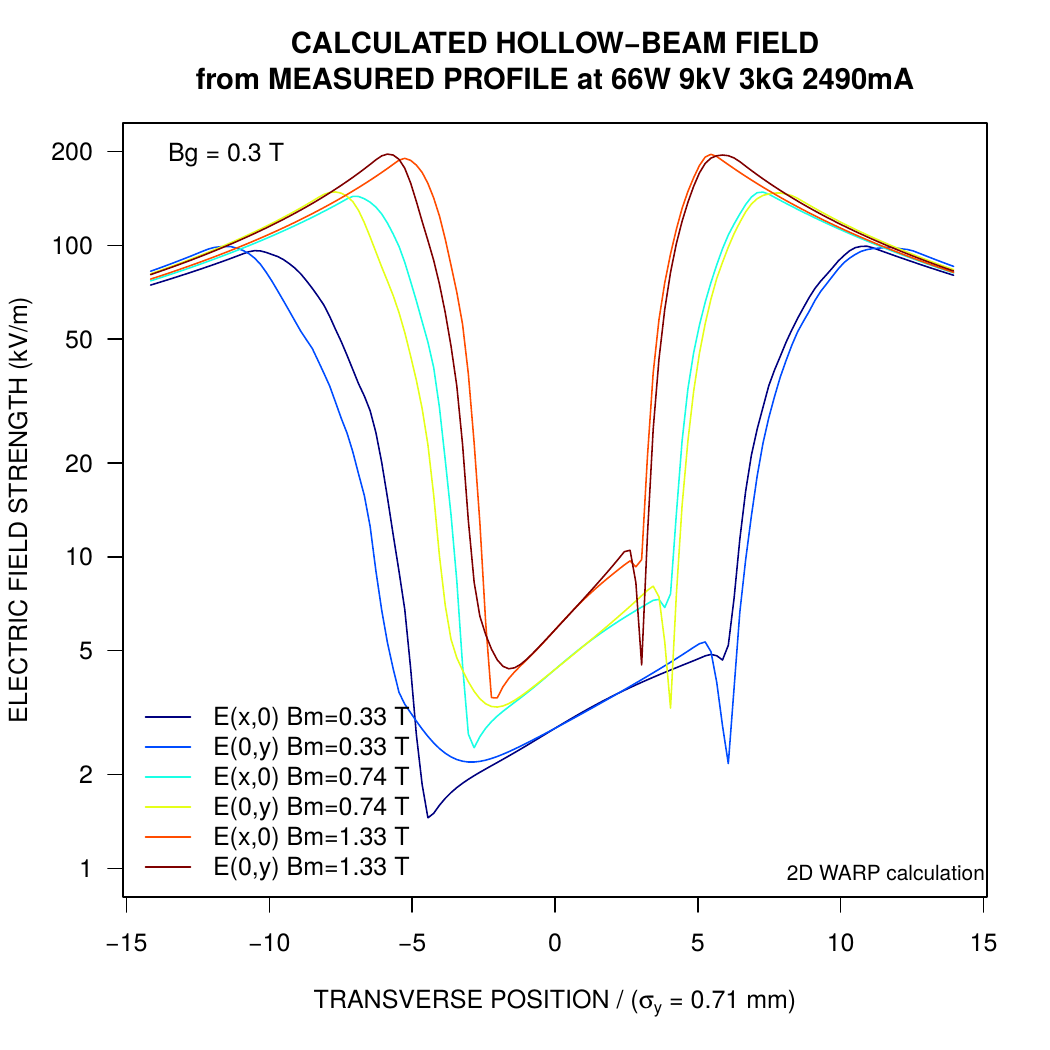
\includegraphics[width=1.0\linewidth]{e-beam_profile.png}
	\caption{Calculated hollow electron beam field from measured profile of 9~kV, 2.49~A e-gun and different main solenoidal fields $Bm$. The field has been calculated using the code WARP \cite{warp}. \textcolor{red}{change $Bm$ to $B_m$ +substitute with new picture.}}
	\label{core:fig:1}
\end{figure}
A first estimate of the residual kick for the HEL design parameters (Table~\ref{tab:hel_param}--\ref{tab:hllhc_param}) with a main solenoid field of $B_{m}=\SI{5}{T}$ can be obtained by scaling the electric field at the center from the measurements and simulations shown in Fig.~\ref{core:fig:1}, yielding:
\begin{equation}\label{eqn:kick_central}
\Delta x', \Delta y'=\q{15}{nrad}
\end{equation}
\textcolor{red}{New gun measurements, can we maybe have a WARP simulation for the new design parameters instead of scaling?}

\section{LHC experiments\label{sec:exp}}
\subsection{Overview of LHC experiments\label{sec:exp_sum}}
The experiments at the LHC presented in this paper were aiming at deriving tolerances on the residual HEL field at the location of the beam core in case of pulsed operation. In total, two experiments were conducted, the first one in 2016 \cite{resexmd2016} and the second one in 2017 \cite{resexmd2017}. The beam and machine parameters for both experiments are summarized in Table~\ref{tab:md_param}.
\begin{table*}
	\caption{\label{tab:md_param}%
		Beam parameters and machine configuration as used in the two resonant excitation experiments in 2016 and 2017 \cite{resexmd2016,resexmd2017}. The plane of the excitation is abbreviated with H for horizontal, V for vertical and H+V horizontal and vertical at the same time.
	}
	\begin{ruledtabular}
		\begin{tabular}{lcc}
			Parameter & Experiment 2017 & Experiment 2016  \\
			\colrule
			beam &\multicolumn{2}{c}{Beam~1} \\
			beam energy &\multicolumn{2}{c}{injection energy, 450 GeV} \\\hline
			single bunch intensity &\multicolumn{2}{c}{$0.7\times10^{11}$} \\
			normalized emittance &\multicolumn{2}{c}{$2.5-3.5~\mathrm{\mu m}$} \\
			$4\sigma$ bunch length & \multicolumn{2}{c}{1.3~ns}\\
			$1\sigma$ bunch length & \multicolumn{2}{c}{9.7~cm}\\
			number of bunches & $3\times72=216$ bunches & $12\times4=48$ single bunches\\
			& (+ 1 pilot + 12 nominal) & \\\hline
			injection optics, $\beta^*=11$~m & standard optics 2017 & standard optics 2016\\
			Landau damping octupoles  & \multicolumn{2}{c}{$I_{\mathrm{MO}}=\pm19.6~\mathrm{A}$, explicitly +19.6 A for MOF circuit and}\\
			& \multicolumn{2}{c}{-19.6~A for MOD circuit (standard 2016 settings)}\\\hline
			working point $(Q_x,Q_y)$ & (62.27,60.295) & (64.28,59.31)\\
			chromaticity $(Q'_x,Q'_y)$ & \multicolumn{2}{c}{(+15,+15)}\\\hline
			pulsing patterns  & $7^{\mathrm{th}}$~turn H,V,H+V;& $7^{\mathrm{th}}$~turn H;\\
			& $8^{\mathrm{th}}$~turn H,V,H+V;& $10^{\mathrm{th}}$~turn V;\\
			& random  H,V,H+V;& \\
		\end{tabular}
	\end{ruledtabular}
\end{table*}
As there is currently no HEL installed in the LHC, the kick on the beam core is emulated by a dipole kick applied with the transverse damper of which more details are given in Section~\ref{sec:adt}. Explicitly, all orders higher than the first order are neglected. Preceding the beam experiments, simulations were performed to identify the most effective pulsing pattern for the $k^{\mathrm{th}}$~turn pulsing (see Sec.~\ref{sec:pattern}) and yield estimates for losses and emittance growth. The two $k^{\mathrm{th}}$~turn pulsing patterns with the largest effect, one $k^{\mathrm{th}}$~turn pulsing pattern with no effect and the random excitation could then be experimentally tested in the LHC limited obviously by the beam time available. To at least test the reproducibility of the results on the example of one pulsing pattern, the $7^{\mathrm{th}}$~turn turn pulsing was tested in the 2016 experiments and then repeated in the 2017. During the experiments the losses were measured with the fast beam current transformers (FBCT) and the emittance and transverse beam profiles with the beam synchrotron radiation telescope (BSRT). The analysis of the BSRT profiles is quite involved and we therefore concentrate in this paper only on the main results. A detailed description of the analysis can be found in \cite{bsrtprofinj} and for the individual experiments in \cite{resexmd2016,resexmd2017}.

\subsection{Excitation with transverse damper and filling scheme\label{sec:adt}}
\textcolor{red}{Daniel's part}
\begin{itemize}
	\item error on amplitude
	\item synchronization of H and V kicker
	\item random noise on amplitude - is there any?
	\item bandwidth - why does the damper not affect the nth turn pulsing????
	\item filling scheme
\end{itemize}

\subsection{Overview of simulations\label{sec:sim}}
For the preparation and interpretation of the experiments two different types of simulations were performed:
\begin{enumerate}
	\item tracking of a Gaussian distribution (Distribution Tracking) to obtain loss rates and emittance growth,
	\item Frequency map analysis (FMA)~\cite{fmalaskar} for the visualization of resonances.
\end{enumerate}
For both simulation types, the tracking code Lifetrac \cite{lifetrac} was used and the simulation parameters are summarized in Table~\ref{tab:sim_param}. Further details on the simulations can be found in \cite{md_sim_hel_res_ex_fitterer,md_sim_hel_res_ex_fitterer_update}.
\begin{table}[b]
	\caption{\label{tab:sim_param}%
		Summary of simulation parameters for the Distribution Tracking and FMA analysis. For details see \cite{md_sim_hel_res_ex_fitterer,md_sim_hel_res_ex_fitterer_update}.
	}
	\begin{ruledtabular}
		\begin{tabular}{lcc}
			Parameter & Distribution Tracking & FMA \\
			\colrule
			beam &\multicolumn{2}{c}{Beam~1} \\
			beam energy &\multicolumn{2}{c}{450 GeV} \\
			emittance & $2.5~\mu$m or $3.5~\mu$m& $2.5~\mu$m\\
			$4\sigma$ bunch length & \multicolumn{2}{c}{1.3~ns}\\
			$1\sigma$ bunch length & \multicolumn{2}{c}{9.7~cm}\\
			particle & 6D Gaussian & equally spaced grid\\
			distribution &  distribution & in $x,y$ up to $10~\sigma$\\
			&  ($10^4$ particles) & with $\frac{\Delta p}{p_0}=0$\\
			turns tracked & $10^6$ turns & $10^4$ turns \\\hline
			optics & \multicolumn{2}{c}{2016 or 2017 injection optics,}\\
			& \multicolumn{2}{c}{$\beta^*=11$~m}\\
			machine  & standard errors & no errors \\
			imperfections &with $a_1=b_1=a_2=0$\footnote{Orbit errors are disabled due to different implementation of the $a_1,b_1,a_2$ errors in Lifetrac and MAD-X. $b_2$ errors are adjusted to yield an average (over 60 seeds) peak $\beta$-beat of 15\% as expected from optics measurements in the LHC.} &  \\
			octupoles  & \multicolumn{2}{c}{$I_{\mathrm{MOF}}=+19.6~\mathrm{A}$, $I_{\mathrm{MOD}}=-19.6~\mathrm{A}$}\\
			tune $(Q_x,Q_y)$ & \multicolumn{2}{c}{(64.28,59.31) for 2016,}\\
			& \multicolumn{2}{c}{(62.27,60.295) for 2017}\\
			chromaticity & \multicolumn{2}{c}{(+15,+15)}\\
			 $(Q'_x,Q'_y)$ & & \\\hline
			 transv. aperture & $5.7~\sigma$ & - \\
			 long. aperture & $10~\sigma$ & - \\
		\end{tabular}
	\end{ruledtabular}
\end{table}

\subsection{Simulation and experimental results\label{sec:simex}}
In the following we will summarize the simulation and experimental results. We will jump forth and back between both as the experimental results are best understood on the base of the simulations.

In summary, the most efficient pulsing patterns and the general tendency of the distribution changes could be successfully predicted in simulations (Sec.~\ref{sec:pattern}). Quantitative predictions of loss rates and emittance growth though failed as both observables are influenced also by the natural noise present in the LHC like ground motion and tune modulation. At injection this natural noise component is now known for the LHC. The observed effect is then the result of the interaction of the external excitation with the natural noise present.

In case of a resonant excitation, the beam distribution adjusts to a new equilibrium distribution. In the presence of only a resonant excitation, this distribution is stable and stays unchanged. If the resonant excitation interacts with the natural noise sources, the beam distribution still changes to a new equilibrium distribution but this change is also accompanied by a resonant excitation amplitude dependent emittance growth. Both effects were experimentally observed in case of the $10^{\mathrm{th}}$~turn pulsing (Sec.~\ref{sec:simex10}).

In case of an excitation with random uniform noise, the shape of the distribution does stay Gaussian. The interaction with the natural noise source then only manifests itself in an underestimation of loss rates and emittance growth (see Sec.~\ref{sec:simexran}). This effect was also studied in more detail in \cite{md1433_noise_top_energy,md_noise_bbLHC} for colliding beams at the LHC.

\subsubsection{Predicting the most efficient pulsing pattern with simulations\label{sec:pattern}}
In order to predict the most efficient pulsing pattern, the loss rate and emittance growth from the Distribution Tracking are compared for the different pulsing patterns. The results for the 2016 optics and tune are shown in Fig.~\ref{fig:patternemit}.

\begin{figure}[h]
	\begin{minipage}[t]{0.49\linewidth}
		\centering
		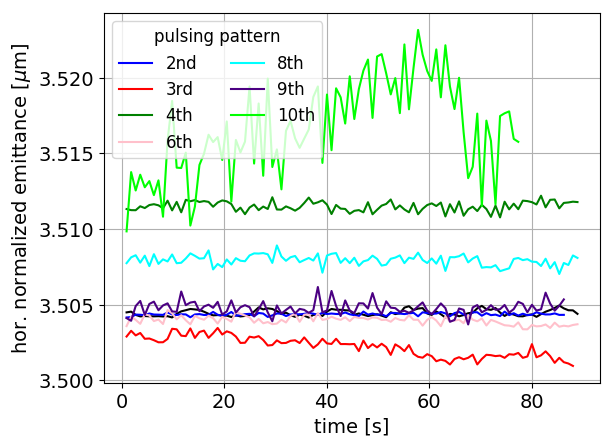
\includegraphics[width=1.0\linewidth]{2016injerrb2u_pattern_3_5um_emit1.png}
	\end{minipage}
	\begin{minipage}[t]{0.49\linewidth}
		\centering
		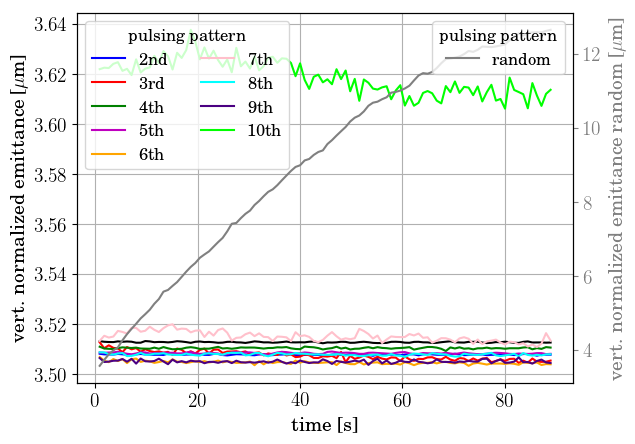
\includegraphics[width=1.0\linewidth]{2016injerrb2u_pattern_3_5um_emit2.png}
	\end{minipage}	
	\caption{\label{fig:patternemit} Horizontal (left) and vertical (right) emittance obtained from simulation results (Distribution Tracking) for different pulsing patterns based on the 2016 injection optics with standard errors. The excitation was applied in both planes with an amplitude of 96~nrad.}
\end{figure}
Only for the $10^{\mathrm{th}}$~turn pulsing and random excitation a considerable emittance growth is visible. For the $10^{\mathrm{th}}$~turn pulsing the vertical emittance also appears to start at an increased initial value and then stays almost constant. This behavior is due to the adjustment of the beam distribution during the first $10^4$ turns to a new equilibrium distribution. Further details on this adjustment will be given in Sec.~\ref{sec:simex10}. As the beam distribution is only dumped every $10^4$ turns, this initial fast adjustment manifests itself only in an increased initial emittance value in Fig.~\ref{fig:patternemit}.

\begin{figure}[h]
	\begin{minipage}[t]{0.49\linewidth}
		\centering
		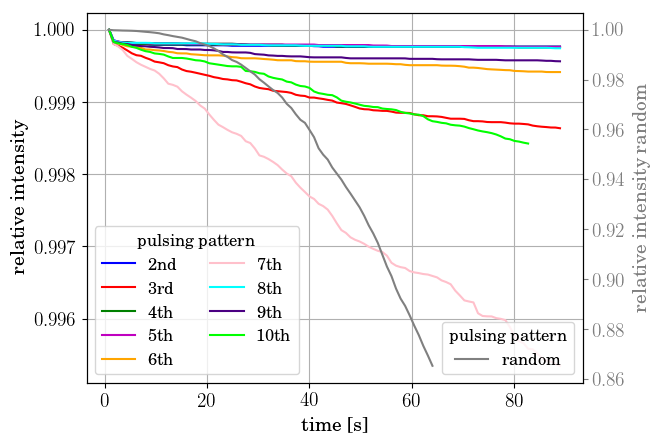
\includegraphics[width=1.0\linewidth]{2016injerrb2u_pattern_3_5um_intensity.png}
	\end{minipage}
	\begin{minipage}[t]{0.49\linewidth}
		\centering
		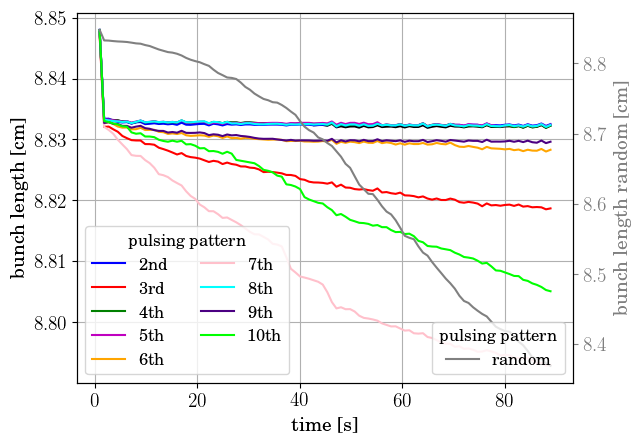
\includegraphics[width=1.0\linewidth]{2016injerrb2u_pattern_3_5um_sigm.png}
	\end{minipage}	
	\caption{\label{fig:patternlosssig} Relative intensity (left) and bunch length (right) obtained from simulation results (Distribution Tracking) for different pulsing patterns based on the 2016 injection optics with standard errors. The excitation was applied in both planes with an amplitude of 96~nrad.}
\end{figure}
The largest losses are observed for $7^{\mathrm{th}}$ and $10^{\mathrm{th}}$~turn pulsing and random excitation. As the bunch length decreases accordingly, the losses are mostly associated to off-momentum particles.

The sensitivity to the $7^{\mathrm{th}}$ and $10^{\mathrm{th}}$~turn pulsing is also observed in absence of machine errors in which case the only source of non-linearities are the strong sextupoles and octupoles \cite{md_sim_hel_res_ex_fitterer}. The FMA analysis shown in Fig.~\ref{fig:patternfma} reveals that 
the $7Q_x$ resonance is excited in case of the $7^{\mathrm{th}}$~turn pulsing and the $10Q_x$ and $10Q_y$ resonance in case of the $10^{\mathrm{th}}$~turn pulsing.
\begin{figure}[h]
	\begin{minipage}[t]{0.49\linewidth}
		\centering
		no excitation
		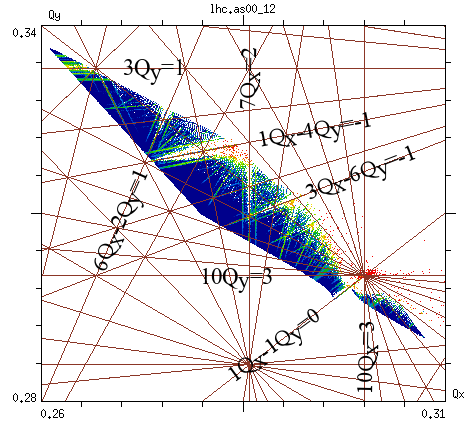
\includegraphics[width=1.0\linewidth]{2016injnocolc15o+19_6noerru_dp0_ord10_annotate.png}
	\end{minipage}
	\begin{minipage}[t]{0.49\linewidth}
		\centering
		$10^{\mathrm{th}}$ H+V
		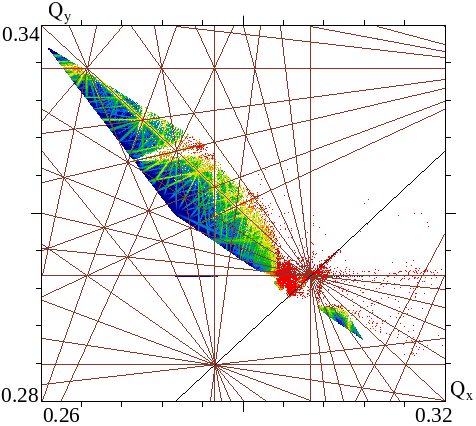
\includegraphics[width=1.0\linewidth]{2016injnocolc15o+19_6noerrut10skhv_dp0_ord10.png}
	\end{minipage}	
	\begin{minipage}[t]{0.49\linewidth}
		\centering
		$7^{\mathrm{th}}$ H
		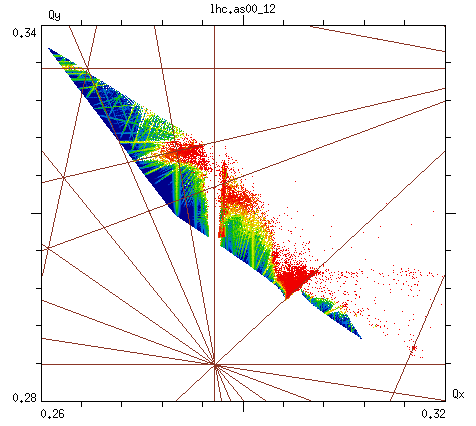
\includegraphics[width=1.0\linewidth]{2016injnocolc15o+19_6noerrut7skh_dp0_ord7.png}
	\end{minipage}	
	\begin{minipage}[t]{0.49\linewidth}
		\centering
		$7^{\mathrm{th}}$ V
		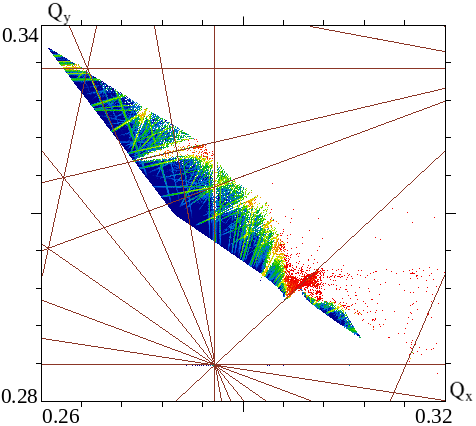
\includegraphics[width=1.0\linewidth]{2016injnocolc15o+19_6noerrut7skv_dp0_ord7.png}
	\end{minipage}
	\caption{\label{fig:patternfma} FMA analysis for $7^{\mathrm{th}}$ and $10^{\mathrm{th}}$~turn pulsing based on the 2016 injection optics with no machine errors. The excitation is 120~nrad in the corresponding plane. The absence of a strong excitation of any resonance in case of $7^{\mathrm{th}}$~turn pulsing only in V and the strong excitation in case of pulsing only in H further confirms that indeed the $7Q_x$ resonance is driven. For $10^{\mathrm{th}}$~turn pulsing there is in contrast no significant difference between pulsing only in H, only in V or in H and V.}
\end{figure}

\begin{itemize}
	\item repeat simulations for each kth turn pattern with only b2 errors
	\item show results when adding random noise -> amplitude dependent emittance growth + losses
	\item FMA plot of 7th (2017) -> explain why in H and in V both losses, FMA plot of 10th (2016), FMA plot of 8th and random
	\item beam distribution change for 10th
\end{itemize}
\begin{itemize}
	\item 7th turn: small emittance but high losses
	\item 8th turn: almost no effect
	\item 10th turn: adjustment of distribution -> emittance growth + small losses
	\item random: constant filamentation -> emittance growth + later strong losses when beam hits aperature
	
\end{itemize}

\subsubsection{7th turn pulsing\label{sec:simex7}}
\subsubsection{10th turn pulsing\label{sec:simex10}}
\subsubsection{8th turn pulsing\label{sec:simex8}}
\subsubsection{random excitation\label{sec:simexran}}

\section{Summary\label{sec:sum}}

\begin{acknowledgments}
We wish to acknowledge Roderik Bruce and Gianluca Valentino for there very helpful suggestions in preparing the experiment at the LHC and we would like to thank all participants of the experiment for helping acquire the data presented in this paper. We would like to acknowledge Dmitry Shatilov for his help with the Lifetrac code, and St\'{e}phane Fartoukh, Riccardo De Maria and Rogelio Tomás for their help with generating the appropiate optics model. We are grateful also for the support from the beam instrumentation team, in particular Enrico Bravin and Georges Trad, with the BSRT and are thankful for the collaboration with St\'{e}phania Papadopoulou and Fanouria Antonio for the analysis of the BSRT profiles.
\end{acknowledgments}

\appendix

\section{Appendixes}


\bibliography{bibliography}% Produces the bibliography via BibTeX.

\end{document}
%
% ****** End of file apssamp.tex ******
